%% LyX 2.1.3 created this file.  For more info, see http://www.lyx.org/.
%% Do not edit unless you really know what you are doing.
\documentclass[10pt,twocolumn,english]{IEEEtran}
\usepackage[T1]{fontenc}
\usepackage[latin9]{inputenc}
\usepackage[a4paper]{geometry}
\geometry{verbose,tmargin=2.2cm,bmargin=2.3cm,lmargin=1.3cm,rmargin=1.1cm,headheight=1.5cm,headsep=1cm,footskip=1.5cm}
\setlength{\parskip}{\smallskipamount}
\setlength{\parindent}{0pt}
\usepackage{units}
\usepackage{amsmath}
\usepackage{graphicx}

\makeatletter

%%%%%%%%%%%%%%%%%%%%%%%%%%%%%% LyX specific LaTeX commands.
%% A simple dot to overcome graphicx limitations
\newcommand{\lyxdot}{.}


%%%%%%%%%%%%%%%%%%%%%%%%%%%%%% User specified LaTeX commands.
\usepackage[nospace]{cite}

\@ifundefined{showcaptionsetup}{}{%
 \PassOptionsToPackage{caption=false}{subfig}}
\usepackage{subfig}
\makeatother

\usepackage{babel}
\begin{document}

\title{A Time and Capture Probability Aware Closed Form Frame Slotted ALOHA
Frame Length Optimization}


\author{Hamed Salah, Hazem A. Ahmed, Joerg Robert, Albert Heuberger \\
Friedrich-Alexander-Universit�t Erlangen-N�rnberg (FAU), Information
Technology (Communication Electronics)\\
\{hamed.kenawy, hazem.a.elsaid, joerg.robert, albert.heuberger\}@fau.de}
\maketitle
\begin{abstract}
Minimizing the reading time in dense Radio-Frequency Identification
(RFID) networks is a critical issue. Commonly used RFID systems are
based on Frame Slotted ALOHA (FSA) for tag anti-collision management.
The usual approach for improved reading times with large tag populations
is the optimization of the number of slots per frame. In real RFID
systems, the slot duration depends on the slot type (i\@.e\@. idle,
successful, or collided). In addition, collided slots might be converted
to successful slots by capturing the strongest transponder, i\@.e\@.
the so-called capture effect. Recent publications have proposed numerical
solutions for obtaining the optimum frame length under these assumptions.
The authors employ numerical solutions that require Multi-dimensional
look-up tables for obtaining the optimum frame length. In this paper
we propose a closed form solution for the analytical calculation of
the optimum frame length. The proposed solution gives a novel closed
form equation for the frame length considering the different slot
durations and the capture effect. Moreover, the paper presents a new
method to calculate the capture probability per frame. Simulations
indicate that the proposed solution gives accurate results for all
relevant parameter configurations without any need for Multi-dimensional
look-up tables. \pagenumbering{gobble}
\end{abstract}


\section{INTRODUCTION}

\IEEEPARstart{O}{ver} the recent years, the number of applications
that use Radio-Frequency Identification (RFID) has increased, and
that number will further grow in the near future. One main application
is the area of logistics, where e\@.g\@. hundreds of tags (transponders)
may be closely placed on pallets. This naturally requires fast RFID
readers in order to not slow down the delivery process of the actual
goods. Commonly used RFID standards in the area of logistics (e\@.g\@.
ISO 18000-6C \cite{standard}) base on TDMA (time division multiple
access). In commercial RFID systems, the tags have to be of low price
and simple design. Hence, they neither can sense the channel nor communicate
with the other tags. Thus, there is a certain probability of tag-collisions,
i.e. multiple tags answer simultaneously. This collision probability
increases in dense networks with many tags. Hence, the readers are
responsible for efficiently coordinating the network, and for the
avoidance of collisions using anti-collision algorithms.

The EPCglobal C1 G2 standard \cite{standard} uses an anti-collision
algorithm based on Framed Slotted ALOHA (FSA) \cite{Aloha2_Floerkemeier}.
The reader signals the frame length (i\@.e\@. the number of available
slots in the frame) to the tags. Each tag then randomly assigns itself
to one of the available slots and replies to the reader within this
slot. Using this algorithm, the reader is able to successfully decode
the data in a specific slot if only one tag replies within this slot.
We call this slot type a successful slot. Furthermore, we have empty
slots (i\@.e\@. no tag replies) and collided slots (i\@.e\@. multiple
tags reply). Due to collisions the reader is not able to identify
all tags in one frame. Hence, it has to use multiple frames to read
all tags. As a tag is deactivated after its successful reading, the
number of tags will decrease from frame to frame and all parameters
have to be adjusted.

The conventional definition of the reading efficiency $\eta_{conv}$
for FSA w\@.r\@.t\@. a single frame is equivalent to the expected
number of successful slots $S$ divided by the summation of the expected
number of empty $E$, successful $S$, and collided $C$ slots.

For a given number of tags $n$ and a frame length of $L$ slots,
the main goal is finding the optimal frame length $L$, which maximizes
the reading efficiency $\eta_{_{conv}}$ \cite{Aloha2_Floerkemeier}.
The reading efficiency $\eta_{_{_{conv}}}$ is maximized to $\eta_{_{_{conv}}}=36\%$
for $L=n$ \cite{Aloha2_Floerkemeier}. However, this assumption is
not precise, as it does not take into consideration the near-far problem
\cite{near_far1}, which is very common in passive RFID systems. A
tag that is close to the reader would reply with a significantly higher
level than other tags that are more distant. In many cases, the reader
would be able to decode the closest tag, even in case of a collided
slot. This effect is the so-called capture effect. Another important
aspect that has to be taken into consideration is the duration of
the slots. The conventional FSA anti-collision algorithms assumes
identical durations of empty, successful, and collided slots. However,
in actual RFID systems these durations differ significantly between
the different slot types \cite{4_1_closed_form_Lopt_not_accurate}.

According to the literature we can divide the previous research for
the optimization of the frame length into three different groups:

The first group considered only the capture probability for the frame
length optimizations, such as \cite{Capture_2011}. The authors proposed
a closed form equation for the optimum frame length maximizing the
reading throughput per frame.

The second group considered only the different slot durations, such
as \cite{4_1_closed_form_Lopt_not_accurate,optimizin_total_latency}.
In \cite{optimizin_total_latency} the authors have optimized the
total latency to read a bunch of tags. However, no closed form solution
for the optimum frame length was derived. They calculate the optimum
frame length numerically. Only \cite{4_1_closed_form_Lopt_not_accurate}
proposed a closed form equation for the optimum frame length taking
into consideration the different slot durations. However, the authors
did not take into their consideration the effect of the capture probability.
Additionally, the equation uses the Lambert-W function that does not
exist in an explicit form.

Finally, the third group considered the different slot durations and
the capture effect, such as \cite{Capture_time_2015,Ref_4_4_2013_Cap_time,2012_curve_fitting}.
Both \cite{Capture_time_2015,Ref_4_4_2013_Cap_time} gave numerical
solutions for the optimum frame length versus the capture probability
and the number of tags. The main problems of their numerical solutions
occur when taking into account the multiple degrees of freedom: the
solutions require a complex multidimensional look-up table that has
to consider all possible degrees of freedom. \cite{2012_curve_fitting}
uses curve fitting to find a closed form solution for the optimum
frame length at a specific capture probability and timing. However,
this solution can not be generalized for all values of slot's timing
and capture probabilities.

In this work, we will derive a closed form solution for the optimum
frame length by optimizing the reading throughput per frame that does
not require any look-up table \cite{Capture_time_2015,Ref_4_4_2013_Cap_time}.
In addition, we take into consideration the capture effect and the
different slot durations. The capture probability takes a value between
$0$ and $1$, and the ratio between the empty and collided slot varies
between $0.18$ and $0.7$ based on the derived formula in section
IV, so two dimensional search is needed to calculate the frame length
numerically which is time consuming in a critical time application
like RFID. Moreover, we will clarify how we calculate the capture
probability based on the physical layer. Afterwards, we will clarify
the effect on the optimum frame length calculations due to the estimation
error of the capture probability. This paper is organized as follows:
Section II presents our system model and considers the different slot
durations and the capture effect. In section III, we analytically
derive a new closed form equation for the optimal frame length based
on the Time and Capture Probability Aware FSA. Finally, we show how
we estimate the capture probability and calculate the value of the
slot duration constant before proving our derivations by comparing
our analytical equations to numerical results.


\section{SYSTEM MODEL WITH DIFFERENT SLOT DURATIONS CONSIDERING THE CAPTURE
EFFECT}

In this section we introduce the Time and Collision Recovery Aware
reading efficiency $\eta_{_{TCA}}$. The main properties for this
efficiency are the consideration of the different slot durations and
the capture probability. Firstly, we consider the different slot durations.
The new time aware reading efficiency is then given by:

{\footnotesize{}
\begin{equation}
\eta_{_{TA}}=\frac{S\cdot t_{s}}{E\cdot t_{e}+S\cdot t_{s}+C\cdot t_{c}},\label{eq:TA_efficiency}
\end{equation}
}{\footnotesize \par}

where $t_{e}$, $t_{s}$ and $t_{c}$ are the durations of the empty,
the successful, and the collided slots, respectively. In addition,
{\small{}$E=L\left(1-\frac{1}{L}\right)^{n}$, $S=n\left(1-\frac{1}{L}\right)^{n-1}$},
and {\small{}$C=L-E-S$.}{\small \par}

Adding the capture effect assuming a capture probability $\alpha$,
the actual values of $E$, $S$, and $C$ have to be converted to
$E_{c}$, $S_{c}$ and $C_{c}$, respectively \cite{Capture_2011}.
Their relation is given by:

{\footnotesize{}
\begin{equation}
E_{c}=E,\,S_{c}=S+\alpha\cdot C,\,C_{c}=(1-\alpha)\cdot C.\label{eq:Succ and Coll with cap}
\end{equation}
}{\footnotesize \par}

Basically, collided slots are converted to successful slots with probability
$\alpha$. From (\ref{eq:Succ and Coll with cap}), the time and capture
probability aware efficiency \cite{Capture_time_2015} can then be
written as:

{\footnotesize{}
\begin{equation}
\eta_{_{_{TCA}}}=\frac{t_{s}\cdot S_{c}}{t_{e}\cdot E_{c}+t_{s}\cdot S_{c}+t_{c}\cdot C_{c}}.\label{eq:eff-semi_simple}
\end{equation}
}The goal is now the maximization of $\eta_{_{_{TCA}}}$ for obtaining
the maximum reading efficiency.


\section{DERIVATION OF THE PROPOSED CLOSED FORM SOLUTION FOR THE OPTIMAL FRAME
LENGTH}

In this section we derive the proposed optimal time and capture-aware
frame size $L_{_{TCA}}$ that takes into consideration the different
slot durations and the capture effect. This is achieved by differentiating
the reading efficiency $\eta_{_{_{TCA}}}$ of (\ref{eq:eff-semi_simple})
with respect to the frame length $L$ and equate the result to zero.

Clearly, the frame length $L$ is an integer value. Therefore, differentiating
the equation is not fully correct. However, we will later show that
the resulting error is negligible. According to (\ref{eq:Succ and Coll with cap}),
$E_{c}$, $S_{c}$, and $C_{c}$ are a function of $L$. However,
$t_{e}$, $t_{s},$ $t_{c}$ are constants for a given system configuration.
Thus, the equation can be simplified to: 

{\footnotesize{}
\begin{eqnarray}
\frac{(t_{e}E_{c}+t_{s}S_{c}+t_{c}C_{c})t_{s}\frac{d}{dL}(S_{c})-t_{s}S_{c}\frac{d}{dL}(t_{e}E_{c}+t_{s}S_{c}+t_{c}C_{c})}{(t_{e}E_{c}+t_{s}S_{c}+t_{c}C_{c})^{2}}\\
=0.\nonumber 
\end{eqnarray}
}{\footnotesize \par}

After multiplying both sides by the denominator and dividing by $t_{s}$
(non-zero constant), and subtracting the term, which is multiplied
by $t_{s},$ the equation results in:

{\footnotesize{}
\begin{equation}
\left(t_{e}E_{c}+t_{c}C_{c}\right)\frac{d}{dL}(S_{c})=S_{c}\frac{d}{dL}\left(t_{e}E_{c}+t_{c}C_{c}\right).\label{eq:simple differentiation}
\end{equation}
}{\footnotesize \par}

Then, the substitution by the values of $E_{c}$, $S_{c}$, and $C_{c}$
from (\ref{eq:Succ and Coll with cap}) leads to the final exact equation
for the proposed time and capture probability aware frame length:

{\footnotesize{}
\begin{eqnarray}
(1-\alpha)\cdot(1-\frac{n}{L_{_{TCA}}})+\alpha\cdot C_{t}\cdot\left(1-\frac{1}{L_{_{TCA}}}\right)\label{eq:Lopt comlex expresion}\\
+\left(C_{t}-1\right)\cdot(1-\alpha)\cdot\left(1-\frac{1}{L_{_{TCA}}}\right)^{n} & = & 0,\nonumber 
\end{eqnarray}
}{\footnotesize \par}

where $n$ is the number of tags, and $C_{t}$ is the slot duration
constant defined as $C_{t}=\frac{t_{e}}{t_{c}}$. (\ref{eq:Lopt comlex expresion})
shows the exact relation between the proposed capture and time-aware
optimum frame length $L_{_{CTA}}$ and the number of tags $n$. This
equation takes into consideration the capture effect and the different
slot durations. However, this solution depends on a recursive equation.
For reaching an explicit equation, (\ref{eq:Lopt comlex expresion})
can be expressed as:

{\footnotesize{}
\begin{eqnarray}
(1-\alpha)\cdot(1-\frac{1}{\beta})+\alpha\cdot C_{t}\cdot\left(1-\frac{1}{\beta n}\right)\label{eq:bita equation}\\
+\left(C_{t}-1\right)\cdot(1-\alpha)\cdot\left(1-\frac{1}{\beta n}\right)^{n} & = & 0,\nonumber 
\end{eqnarray}
}{\footnotesize \par}

where $\beta=\frac{L_{TCA}}{n}$. As we are focusing on systems with
a large number of tags $n$, we can use the approximation

{\footnotesize{}
\begin{equation}
\underset{n\rightarrow\infty}{\lim}\left(1-\frac{1}{\beta n}\right)^{n}=e^{-\frac{1}{\beta}},\label{eq:approx_1}
\end{equation}
}{\footnotesize \par}

which simplifies (\ref{eq:bita equation}) to:

{\footnotesize{}
\begin{eqnarray}
(1-\alpha)\cdot\left(1-\frac{1}{\beta}\right)+\alpha\cdot C_{t}\cdot\left(1-\frac{1}{\beta n}\right)\label{eq:first_approx}\\
+(1-\alpha)\cdot\left(C_{t}-1\right)e^{-\frac{1}{\beta}} & = & 0.\nonumber 
\end{eqnarray}
}{\footnotesize \par}

The analysis of (\ref{eq:Lopt comlex expresion}) indicates that the
relevant values for {\footnotesize{}$\beta=\frac{L_{TCA}}{n}$} are
in the region close to one \cite{Ref_4_4_2013_Cap_time}. Hence, we
can develop a Taylor series for $e^{-\frac{1}{\beta}}$ around one
which leads to:

{\footnotesize{}
\begin{equation}
e^{-\frac{1}{\beta}}\simeq1-\frac{1}{\beta}+\frac{1}{2\beta^{2}}.\label{eq:taylor}
\end{equation}
}{\footnotesize \par}

After substituting (\ref{eq:first_approx}) and some additional simplifications,
we get:

{\footnotesize{}
\begin{equation}
\beta^{2}C_{t}-\beta C_{t}(1+\frac{\alpha}{n})-0.5\left(1-\alpha\right)\cdot\left(1-C_{t}\right)=0.\label{eq:quadratic equation}
\end{equation}
}{\footnotesize \par}

As $\frac{\alpha}{n}\ll1,$ (\ref{eq:quadratic equation}) can be
expressed as:

{\footnotesize{}
\begin{equation}
\beta^{2}C_{t}-\beta C_{t}-0.5\left(1-\alpha\right)\cdot\left(1-C_{t}\right)=0.\label{eq:final quadratic equation}
\end{equation}
}{\footnotesize \par}

By solving (\ref{eq:final quadratic equation}) and rejecting the
negative solution we finally reach to the final solution:

{\footnotesize{}
\begin{equation}
L_{_{TCA}}=\frac{n}{2}\left(\left(1-\alpha\right)+\sqrt{\left(1-\alpha\right)^{2}+\frac{2}{C_{t}}\left(1-\alpha\right)\cdot\left(1-C_{t}\right)}\right).\label{eq:closed form}
\end{equation}
}{\footnotesize \par}

As the optimization of (\ref{eq:eff-semi_simple}) is a convex optimization
problem, and there exits only one non-negative solution of (\ref{eq:final quadratic equation}),
(\ref{eq:closed form}) leads to the global optimum. According to
the literature, \cite{Capture_time_2015} is the only work who used
the same performance metric $\eta_{_{_{TCA}}}$to get the optimum
frame length. However, in this work the authors did not propose any
closed form solution and they have to rely on Multi-dimensional look-up
tables. According to the EPCglobal C1 G2 standard \cite{standard},
the proposed frame length in equation (\ref{eq:closed form}) takes
only discrete values of power $2$. Therefore, the possible quantized
values of the optimum frame length can be expressed as:

\begin{equation}
L_{_{QTCA}}=2^{\text{round}\left(\text{log}_{2}L_{TCA}\right)}.\label{eq:closed form quantized}
\end{equation}


We will proof in the simulation results that $L_{QTCA}$ leads to
the optimum solution.


\section{CAPTURE PROBABILITY AND SLOT DURATION CONSTANT CALCULATIONS}

In this section we will discuss in details how can we calculate the
slot duration constant $C_{t}$ and the capture probability from the
physical layer:


\subsection{Slots Duration Constant calculation}

Based on the EPCglobal C1 G2 standard \cite{standard}, the slot duration
constant $C_{t}$ is $C_{t}=\frac{t_{e}}{t_{c}}$, where $t_{e}$
is given by:

{\footnotesize{}
\begin{equation}
t_{e}=T_{QRep}+T_{1}+T_{3}.\label{eq:te}
\end{equation}
}{\footnotesize \par}

Here, $T_{QRep}$ is the query repeat command time, {\small{}$T_{QRep}=3.5\cdot DR\cdot T_{pri}$},
$T_{pri}=\frac{1}{BLF}$, {\small{}$BLF$} is the backscatter link
frequency of the tag reply, and {\small{}$DR$} is the so-called divide
ratio constant that can take the two values{\small{} $DR=8\,\mbox{or}\,\frac{64}{3}$}.
Next, $T_{1}$ is the time from the reader transmission to the tag
response with $T_{1}=\textrm{max}\left\{ DR\cdot T_{pri},\,10\cdot T_{pri}\right\} $.
Finally,$T_{3}$ is the time that the reader waits after $T_{1}$
before issuing another command. As it has no constrains it can be
assumed to be zero.

Next, $t_{c}$ is given by:

{\footnotesize{}
\begin{equation}
t_{c}=T_{QRep}+T_{1}+T_{2}+T_{RN16},\label{eq:tc}
\end{equation}
}{\footnotesize \par}

where $T_{2}$ is the reader response time starting from the end of
the tag response, $T_{2}=6\cdot T_{pri}$, and $T_{RN16}$ is the
duration of the $16$ bits temporary identifier reply of the tag.
It includes $16$ bits data, $6$ bits preamble, $n_{p}$ pilot tones,
i\@.e\@. $T_{RN16}=(22+n_{p})\cdot T_{pri}$.

After substituting (\ref{eq:te}) and (\ref{eq:tc}) in $C_{t}$ equation,
the the final expression of $C_{t}$ is:
\begin{figure}
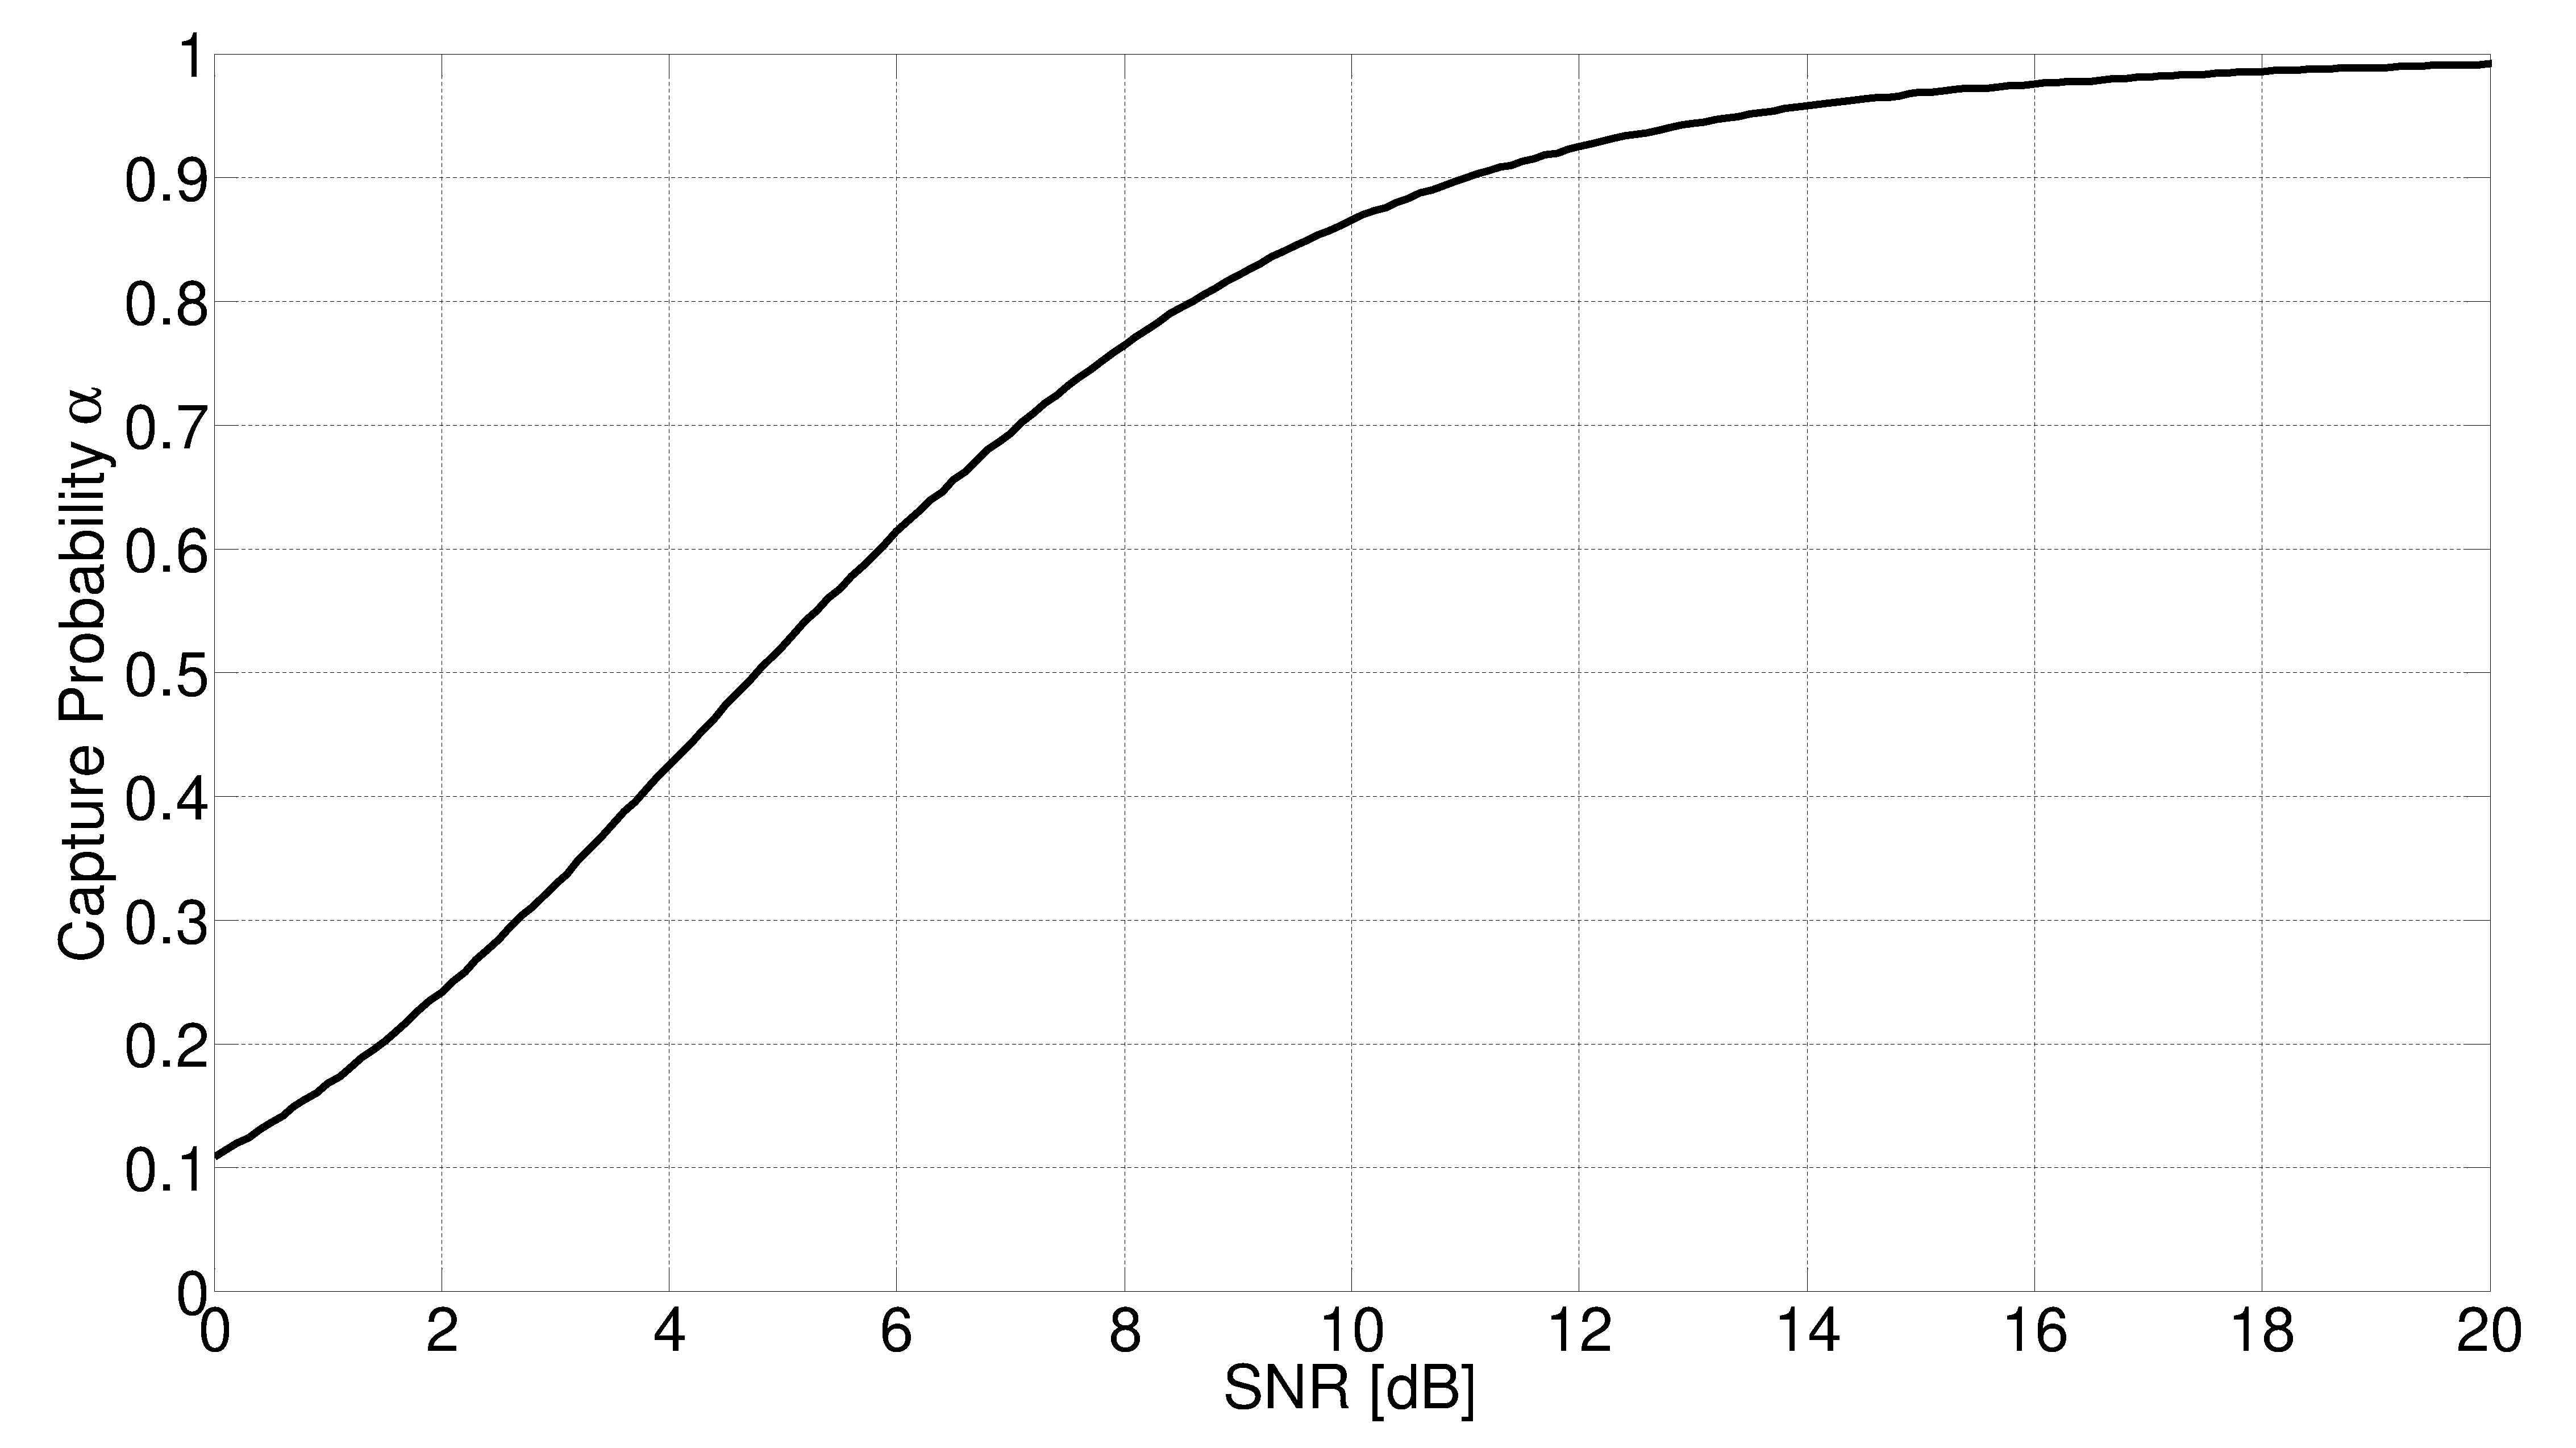
\includegraphics[width=1\columnwidth,height=0.13\paperheight]{capture_probability_vs_SNR}

\protect\caption{Capture probability versus the signal to noise ratio \label{fig:Capture-probability-versus}}
\end{figure}


{\footnotesize{}
\begin{equation}
C_{t}=\frac{3.5\cdot DR+\textrm{max}\left\{ \mbox{\ensuremath{DR}},\,10\right\} }{3.5\cdot DR+\textrm{max}\left\{ DR,\,10\right\} +6+22\cdot M+n_{p}\cdot M}.\label{eq:ct_final}
\end{equation}
}{\footnotesize \par}

where $M$ equals to $1,\,2,\,4$, or $8$ which represents the modulation
types FM0, Miller 2, 4, or 8, respectively.


\subsection{Capture Probability Calculation}

The capture probability varies in the range of $0\leq\alpha\leq1$.
Its value depends on the Signal to Noise Ratio (SNR). In this work,
we measure the SNR for each slot. Then, we calculate the average SNR
per frame. In \cite{2010_Trans_CR}, the authors proposed a method
to capture the strongest tag reply based the physical layer properties.
They have proposed a Bit Error Rate (BER) curve versus the SNR. We
want to calculate the capture probability for a complete collided
RN16 packet, which includes $16$ random successive bits. The BER
is mapped to Packet Error Rate (PER) by simulation as the channel
is not Binary Symmetric Channel (BSC). The capture probability can
be expressed as: $\alpha=(1-PER)$. Figure \ref{fig:Capture-probability-versus}
presents the values of the capture probabilities versus the average
signal to noise ratio per frame. In this work, we calculate the average
capture probability from the corresponding average SNR at the current
frame.
\begin{figure}
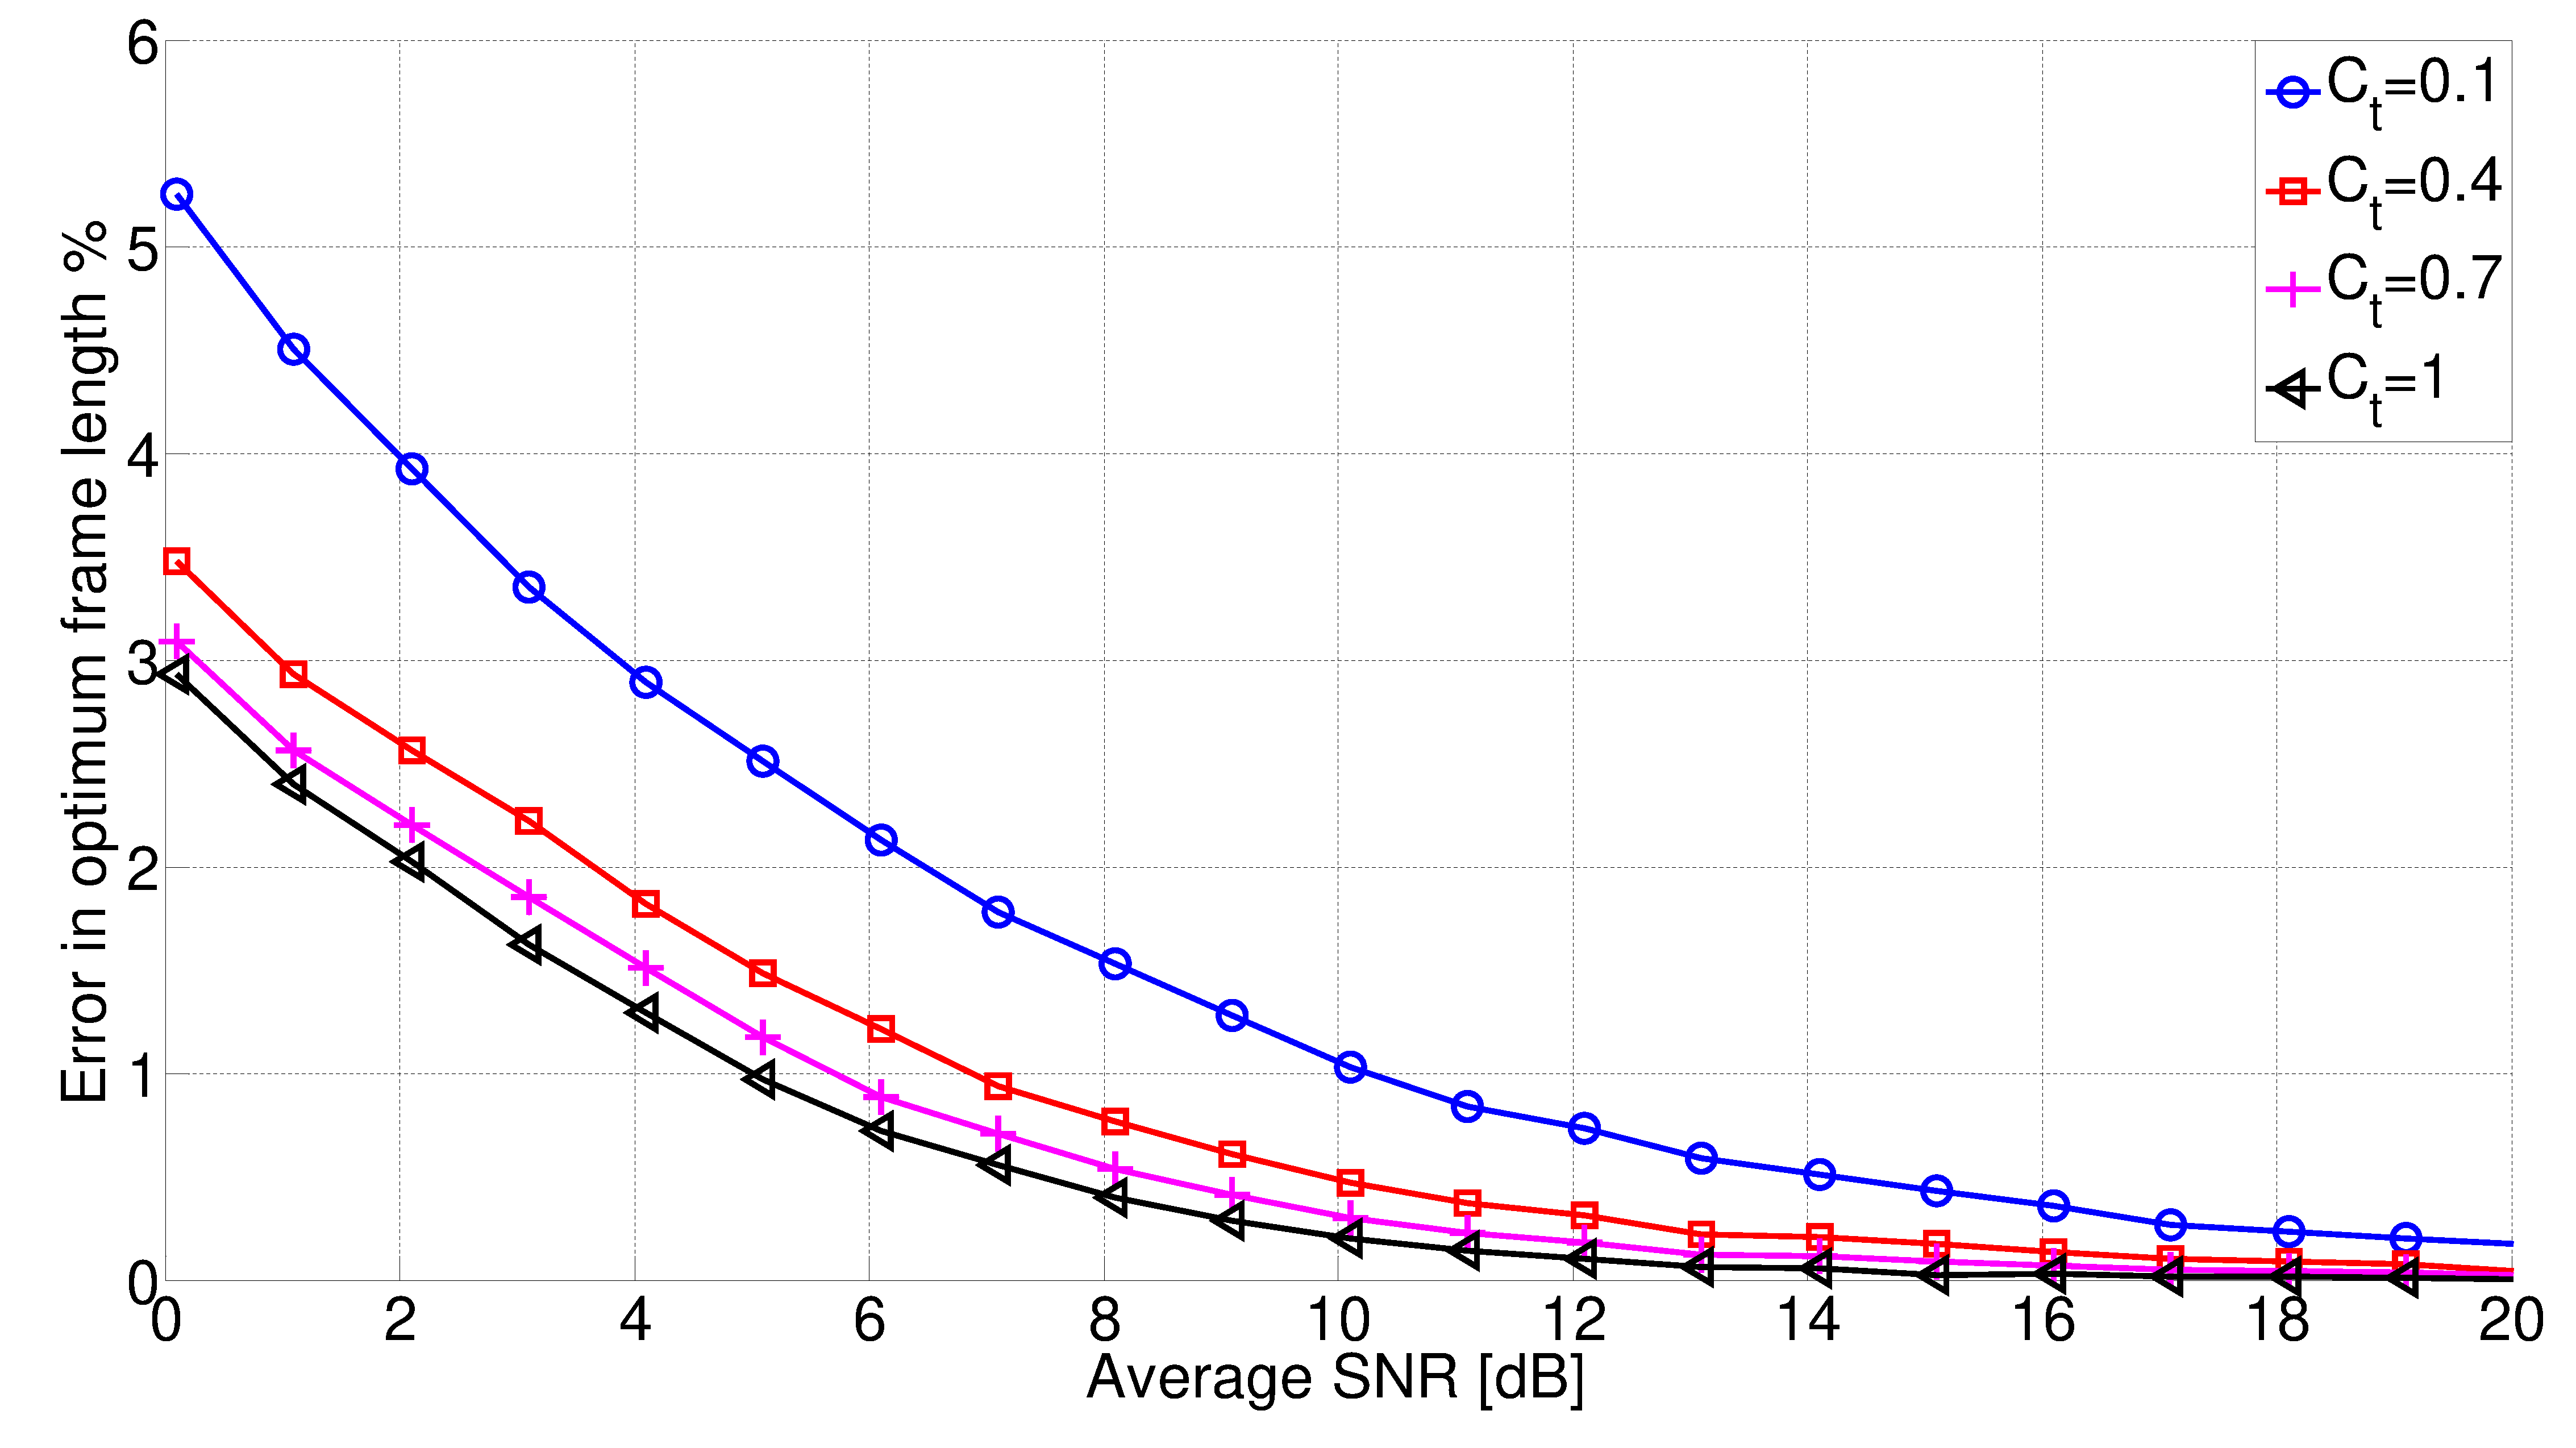
\includegraphics[width=1\columnwidth,height=0.13\paperheight]{Error_in_frame_length}

\protect\caption{Effect of the SNR measurement error on the proposed formula using
sampling rate $f_{s}=\unit[8]{MHz}$, and symbol rate $\unit[640]{kHz}$\label{fig:Effect-of-the} }
\end{figure}



\section{SIMULATIONS RESULTS AND COMPARISONS}

Figure \ref{fig:Effect-of-the} shows the relative error of the proposed
formula (\ref{eq:closed form}) due to the average SNR measurement
error. According to the European standard \cite{standard}, the bandwidth
of the UHF RFID systems is $\unit[4]{MHz}$, so we used a sampling
frequency of $f_{s}=\unit[8]{MHz}$. To clarify the worst case effect
of the estimation error, we used the highest symbol rate $\unit[640]{kHz}$
in this simulations. The SNR per slot is measured at the first part
of each slot $T_{1}$. The average SNR per frame is calculated as
$E\left\{ \frac{\left|h\right|^{2}\cdot x^{2}}{\sigma^{2}}\right\} $
, where $\text{\ensuremath{\sigma}}$ is the standard deviation of
the Additive White Gaussian Noise (AWGN) per slot, and we used normalized
signal power i.e. $E\left\{ x^{2}\right\} =1$ . Based on \cite{2010_Trans_CR},
we assumed that the equivalent channel coefficients $h$ follow Rayleigh
fading. The single Rayleigh channel coefficients are independent zero
mean circularly symmetric complex Gaussian random variables with normalized
energy $E\left\{ \left|h\right|^{2}\right\} =1$, and all tags are
statistically identical, which means all of them experience the same
path loss. Therefore, the average SNR per frame is $E\left\{ \frac{1}{\sigma^{2}}\right\} $.
Afterwards, we get the error in the measured SNR by comparing the
measured value by the nominal one. According to the relation between
the capture probability $\alpha$ and the SNR (shown in figure \ref{fig:Capture-probability-versus}),
and the relation between the proposed optimum frame length and the
capture probability in (\ref{eq:closed form}), the estimation error
of the measured SNR is mapped to an error of the proposed frame length
versus the SNR. Based on Figure \ref{fig:Effect-of-the}, for a constant
value of the slot duration constant $C_{t}$, the error in the frame
length decreases when the SNR increases. Moreover, when the slots
duration constant $C_{t}$ decreases, the error in the proposed formula
increases up to $5\%$ at zero dB SNR, which is negligible.

Now we will compare the proposed closed form equation in (\ref{eq:closed form})
with the numerical results in \cite{Capture_time_2015}. Figure \ref{fig:Non-quantized}
shows the non-quantized optimal frame length of both algorithms for
the full range of the slot duration constant $C_{t}$. Assuming a
fixed number of $n=100$ tags, figure \ref{fig:Non-quantized} indicates
that the proposed closed form approaches the numerical solution for
different $\alpha$ in the full range of $C_{t}$. Due to the proposed
approximations, there are slight differences between the proposed
closed form and the numerical solution, where the numerical is the
exact solution. According to the EPCglobal C1 G2 standard \cite{standard}
the frame length is allowed to take only quantized values (power of
$2$). Figure \ref{fig:Quantized-Frame-Length} shows that the proposed
frame length fully match the numerical solution in the full range
of $C_{t}$. 


\section{CONCLUSIONS}

This paper proposes a novel closed form solution for analytically
calculating the optimum frame length for Frame Slotted ALOHA. We especially
consider the effects of unequal slot durations and the capture probability,
which have to be taken into account for optimizing the reading speed
in real RFID systems. The theoretical derivations lead to a new analytical
optimum frame length equation that can be easily implemented in RFID
readers. The optimum frame length for different slot durations in
addition to the capture effect has been previously addressed in literature.
However, the authors did not derive any any closed form solution for
this problem. Our proposed frame equation gives a direct linear relation
with the number of tags in the reading area instead of using Multi-dimensional
look-up tables. Furthermore, our analytical solution can be used for
further optimizations of RFID systems. Simulation results prove the
correctness of our analytical solution. 
\begin{figure}
\subfloat[Non-quantized Frame Length \label{fig:Non-quantized}]{\protect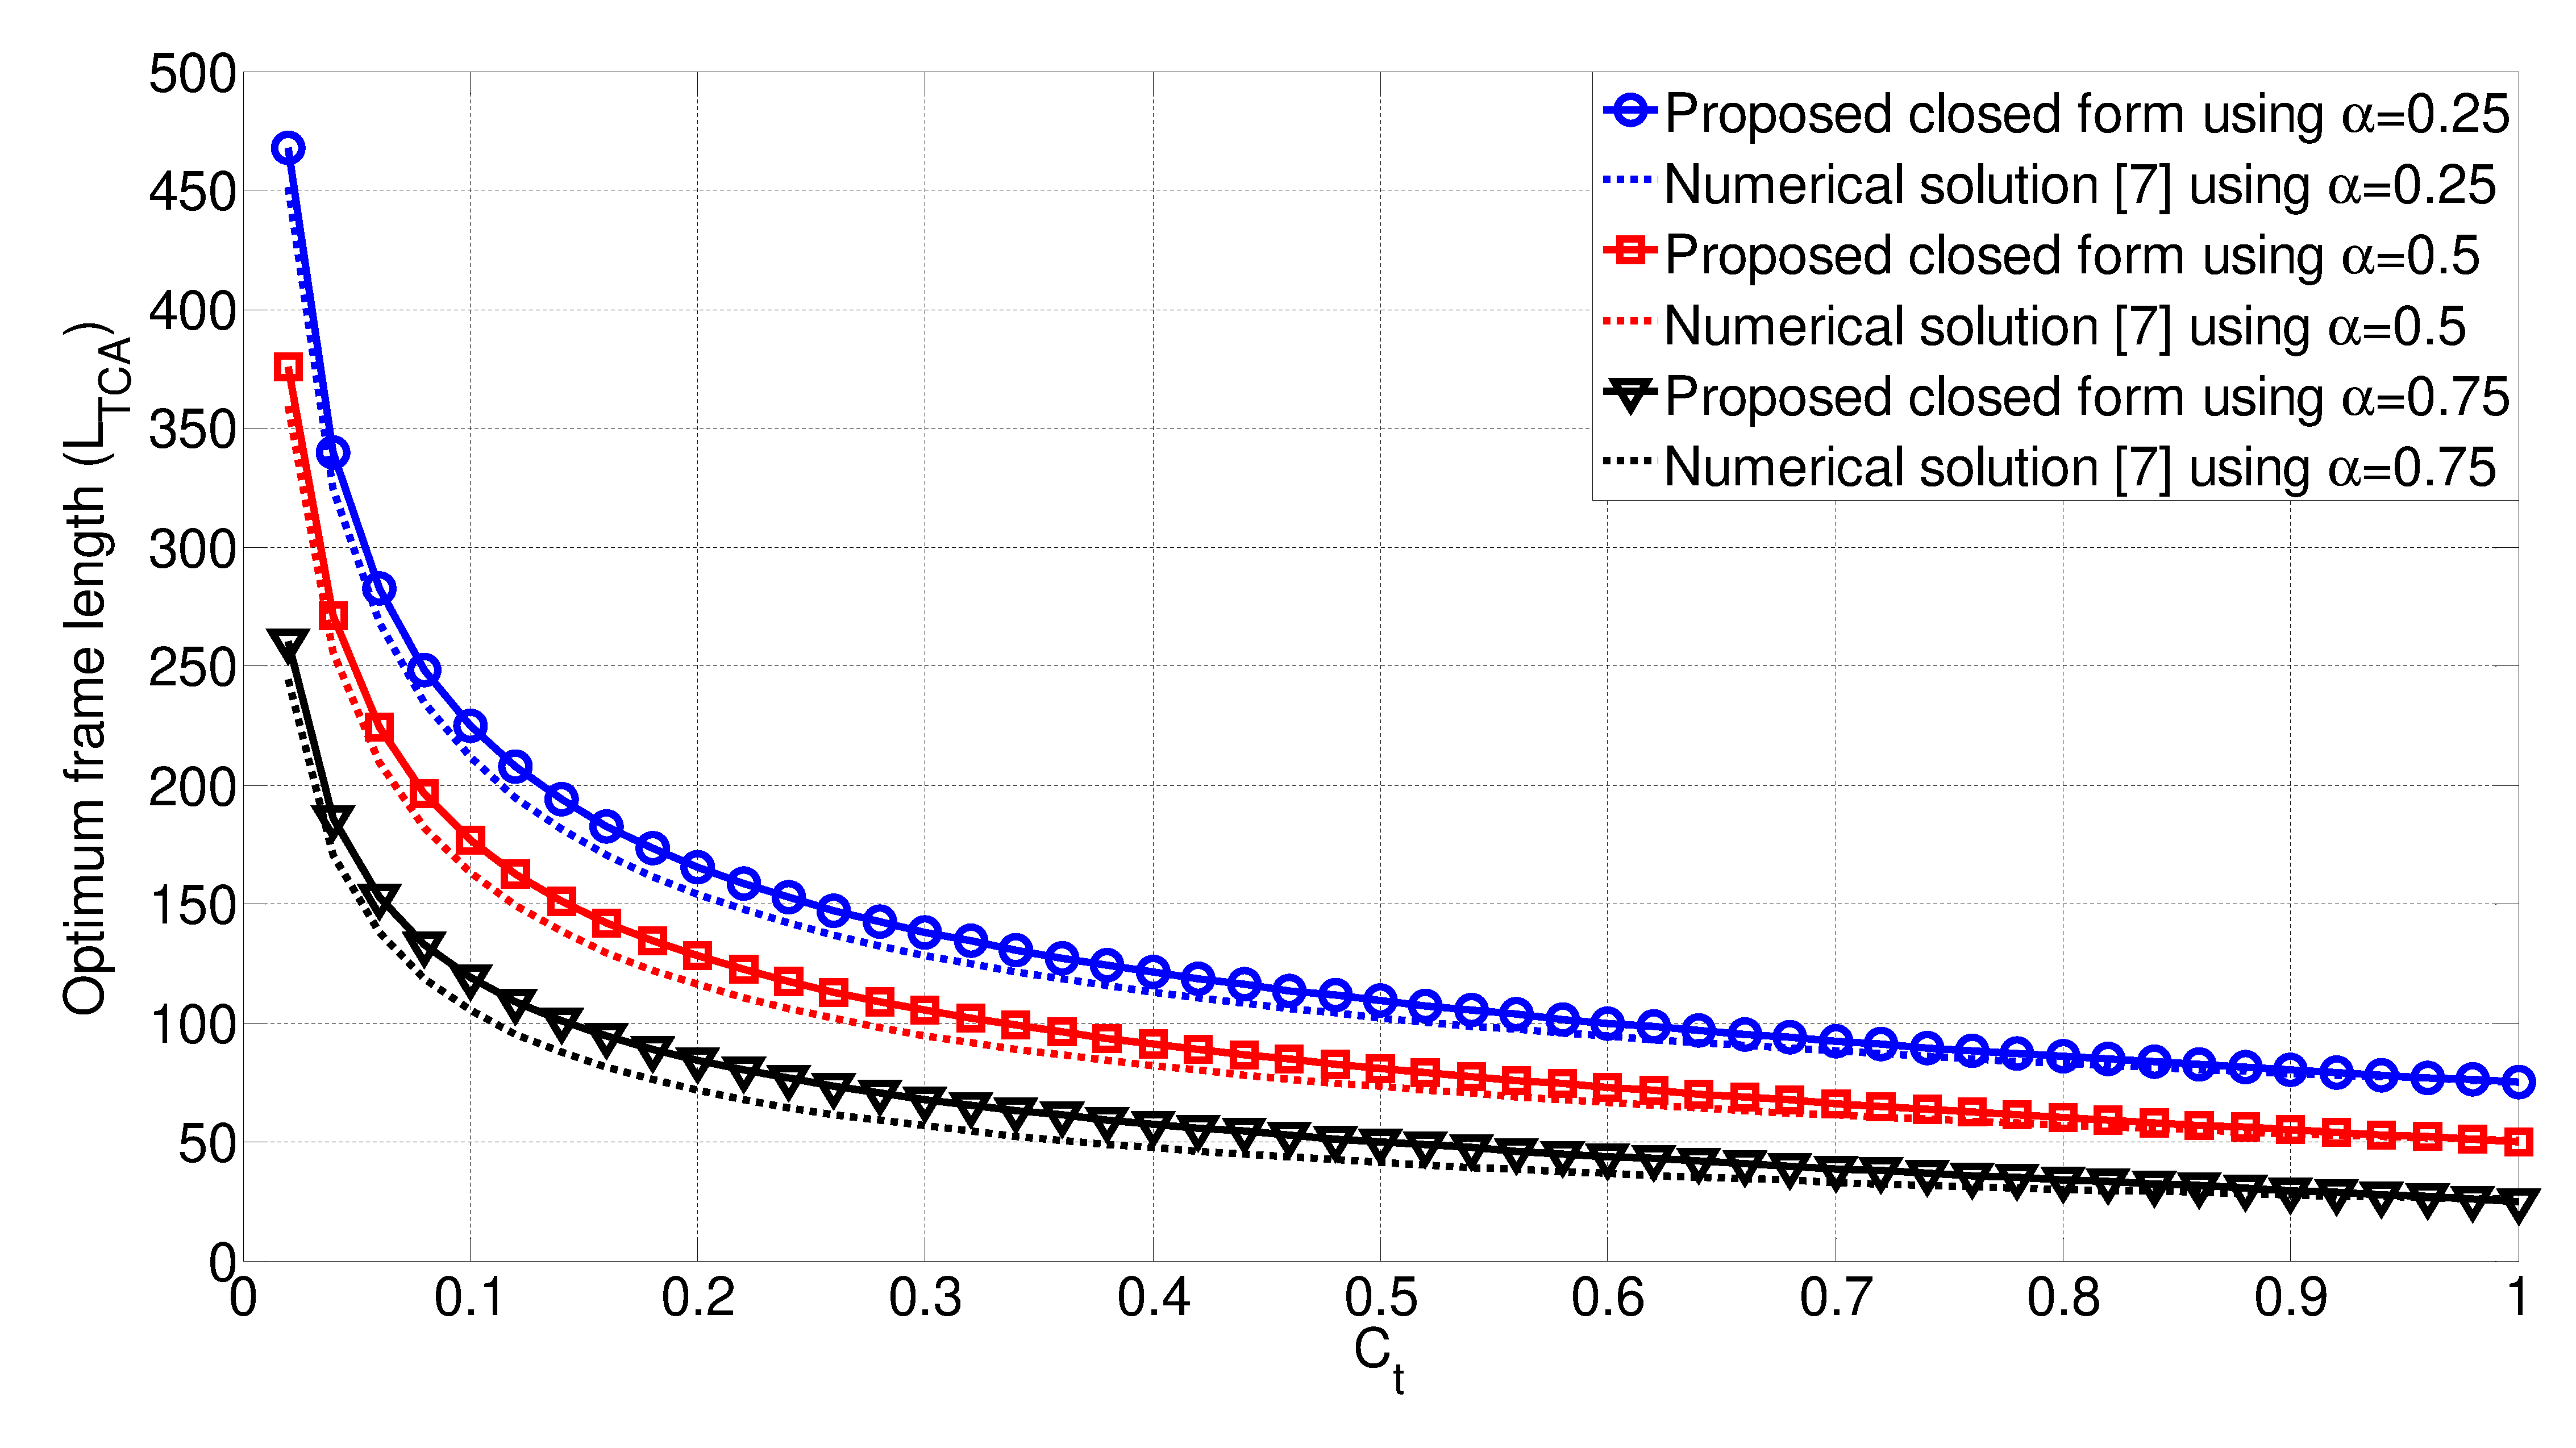
\includegraphics[width=1\columnwidth,height=0.13\paperheight]{Lopt_vs_n_diff_Ct_diff_alpha}

}

\subfloat[Quantized Frame Length \label{fig:Quantized-Frame-Length}]{\protect\includegraphics[width=1\columnwidth,height=0.13\paperheight]{Lopt_vs_Ct_quantized_0\lyxdot 001_0\lyxdot 01_new}

}

\protect\caption{Optimum frame length $L_{_{TCA}}$ as a function of the slot duration
constant $C_{t}$ ($n=100$ tags) for the capture probabilities $\alpha=0.25,\,0.5,\,0.75$.\label{fig:Frame size ct}}
\end{figure}


\bibliographystyle{ieeetr}
\bibliography{Lopt_second_review}

\end{document}
